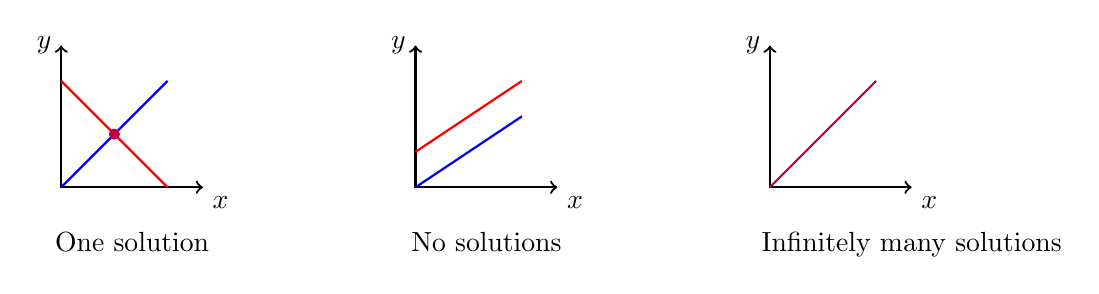
\begin{tikzpicture}[scale=0.9]
    \draw[thick, <->](0,2)--(0,0)--(2,0);
    \draw[thick, red](0,1.5)--(1.5,0);
    \draw[thick, blue](0,0)--(1.5,1.5);
    \draw[fill, purple](0.75,0.75) circle [radius=2pt];
    \node[below right] at (2,0){$x$};
    \node[left] at (0,2){$y$};
    \node[below] at (1,-0.5){One solution};

    \draw[thick, <->](5,2)--(5,0)--(7,0);
    \draw[thick, red](5,0.5)--(6.5, 1.5);
    \draw[thick, blue](5,0)--(6.5,1);
    \node[below right] at (7,0){$x$};
    \node[left] at (5,2){$y$};
    \node[below] at (6,-0.5){No solutions};

    \draw[thick, <->](10,2)--(10,0)--(12,0);
    \draw[thick, purple](10,0)--(11.5, 1.5);
    \node[below right] at (12,0){$x$};
    \node[left] at (10,2){$y$};
    \node[below] at (12,-0.5){Infinitely many solutions};
  \end{tikzpicture}
